\section{Distributed systems}

We implement distributed systems when our system becomes too big to be run from a single computer. Distribution always makes things more complex, so there is no reason to implement it when you don't have to. But in almost every case, you eventually will. 

\subsection{Model}
\begin{itemize}
    \item \textbf{Communication graph} $G$: a directed, two-way graph
      \begin{itemize}
        \item nodes: \nodes{G}
        \item edges: \edges{G}
        \item $\forall (u, v) \in \edges{G}: (v, u) \in \edges{G}$
      \end{itemize}
    \item \textbf{Subgraph} $U_G$:
      \begin{itemize}
        \item nodes: \nodes{U}
        \item edges: $\edges{U} = \{(u, v) | u \in \nodes{U} \land v \in \nodes{U}\}$
      \end{itemize}
    \item \textbf{Inedge border} of $U_G$: $\{(u, v) | u \notin \nodes{U} \land v \in \nodes{U}\}$
    \item \textbf{System} $\mathcal{G}$:
      \begin{itemize}
        \item a communication graph $G$
        \item a program $A$ for each node $n$ of $G$ (we say: $n$ runs $A$) (in the original paper, a program was called a \emph{device})
        \item input to each node $n$ of $G$
        \item behaviour $\mathcal{B_G}$
      \end{itemize}
\end{itemize}

\subsection{Axioms}
\paragraph{The locality axiom} states that a subsystems behaviour is only influenced by its inedge border.
\paragraph{The fault axiom} states that 

\subsection{Theorems}

\subsubsection{Coverings}
Define the \emph{neighborhood} of node $u$ as $\text{nbh}_u = \{ v \in \nodes{G} | (v, u) \in \edges{G} \}$. A graph $S$ \emph{covers} $G$ if there is a mapping $\phi$ from any node $s \in S$ to $u \in G$ that preservers neighborhood, that is: 
$$ \phi: \nodes{S} \to \nodes{G} $$
$$ \forall s \in \nodes{S}: \phi(s) = w \then \phi( \text{nbh}_s ) = \text{nbh}_w $$
Under such a mapping, $S$ looks locally like $G$.

\subsubsection{Byzantine agreement}
\subsubsection{Week agreement}
\subsubsection{Byzantine fireing squad}
\subsubsection{Approximate agreement}
\subsubsection{Clock syncing}


\subsubsection{When timing does and does not matter}
Operations on a single machine have a total order, on distributed machines we can at least hope to acchieve a partial order.
Consider a transition function from one state to another. When is a transition function commutative? That would mean that the timing in which input arrives at a state machine does not matter. We know this is not always true. Just consider the state function $f(s, x) = sx + x$. 
$$ f : S \times X \to S$$
Theorem:
$$ f: \text{some property} \then f(f(s_0, x_0), x_1) = f(f(s_0, x_1), x_0)$$

\subsubsection{flp theorem}

\paragraph{System model} consists of:
\paragraph{In an asynchronous system, a server-failure can alter the outcome} This is
\paragraph{When you are at a bivalent state, you can delay a message such that you end up at a bivalent state again} This means that you can forever postpone the system from ever reaching a conclusion. 

\subsubsection{CAP-Theorem}


\subsection{Important alogrithms}

\subsubsection{one-, two- and tree-phase commit}

\subsubsection{paxos algorithm}

\subsubsection{raft algorithm}

\subsubsection{map reduce algorithm}
where in map reduce is the window of failure according to flp?


\subsection{Databases}

\subsubsection{ACID}
A transaction is a sequence of database operations that can be considered one independent, coherent unit of work. Database transaction should have the ACID-properties:
\begin{itemize}
    \item Atomicity
    \item Consistency
    \item Isolation
    \item Durability
\end{itemize}

If a distributed database provides the acid-properties, then it must chose consistency over availability according to the cap theorem. A available database cannot provide acid-transactions. 

\subsubsection{NoSQL Database types}
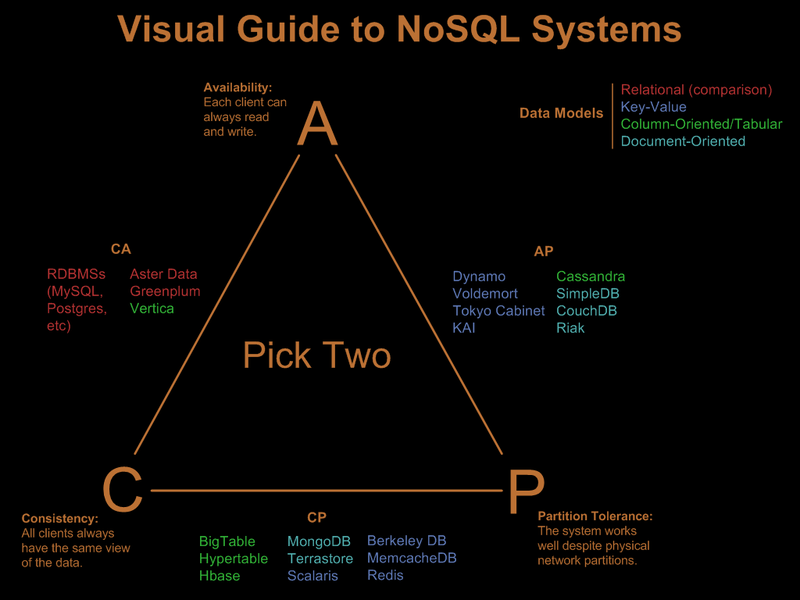
\includegraphics[scale=0.5]{images/cap_choice.png}


\subsubsection{Normalisation}
Normalisation is a way of structuring a relational database such that logical errors are minimized. 

\begin{lstlisting}[language=python]
from DB import DB


class DictOfSets:
    data = {}

    def addData(self, d):
        for row in d:
            if row[0] in self.data:
                self.data[row[0]].add(row[1])
            else:
                self.data[row[0]] = set([row[1]])

    def addVals(self, v):
        for row in v:
            if row[0] in self.data:
                self.data[row[0]].add(row[1])

    def addKeys(self, k):
        for key in k:
            if not key in self.data:
                self.data[key] = set()

        

class DBAbstr:
    host = '10.173.202.110'
    user = 'lesen'
    password = ''
    database = 'gkd_chemie'
    
    def doQuery(self, query):
        result = []
        with DB(self.host, self.user, self.password, self.database) as db:
            result = db.queryToArray(query)
        return result


class SetTable(DBAbstr):
    vals = []

    def __init__(self, tableName, key):
        self.tableName = tableName
        self.key = key

    def getVals(self):
        if self.vals:
            return self.vals
        query = "select {0} from {1} group by {0}".format(self.key, self.tableName)
        result = self.doQuery(query)
        self.vals = result
        return result


class RelTable(DBAbstr):
    leftVals = DictOfSets()
    rightVals = DictOfSets()

    def __init__(self, tableName, setA, translKeyA, setB, translKeyB):
        self.tableName = tableName
        self.setA = setA
        self.translKeyA = translKeyA
        self.setB = setB
        self.translKeyB = translKeyB

    def getLeftVals(self):
        if self.leftVals.data:
            return self.leftVals.data
        query  = "select a." + self.setA.key + ", c." + self.setB.key + " "
        query += "from " + self.setA.tableName + " as a "
        query += "left join " + self.tableName + " as b on b." + self.translKeyA + " = a." + self.setA.key + " "
        query += "left join " + self.setB.tableName + " as c on c." + self.setB.key + " = b." + self.translKeyB + " "
        query += "group by a." + self.setA.key + ", c." + self.setB.key
        result = self.doQuery(query)
        self.leftVals.addData(result)
        return result

    def getRightVals(self):
        if self.rightVals.data:
            return self.rightVals.data
        query  = "select a." + self.setB.key + ", c." + self.setA.key + " "
        query += "from " + self.setB.tableName + " as a "
        query += "left join " + self.tableName + " as b on b." + self.translKeyB + " = a." + self.setB.key + " "
        query += "left join " + self.setA.tableName + " as c on c." + self.setA.key + " = b." + self.translKeyA + " "
        query += "group by a." + self.setA.key + ", c." + self.setB.key
        result = self.doQuery(query)
        self.rightVals.addData(result)
        return result





class Relation:
    vals = DictOfSets()     # x  ->  f(x) = y
    invVals = DictOfSets()  # y  ->  f^-1(y) = x

    def __init__(self, setTableX, setTableY, relTable):
        self.setTableX = setTableX
        self.setTableY = setTableY
        self.relTable = relTable

    def checkTransitive(self):
        pass

    def checkBijective(self):
        """ One-to-one and onto """
        return self.checkSurjective and self.checkInjective

    def checkSurjective(self):
        """ Onto: For any y in Y, there is a x in X: y = f(x) """
        invValsData = self.getInvValsData()
        for y in invValsData:
            if len(invValsData[y]) == 0:
                return False
        return True

    def checkInjective(self):
        """  Ont-to-One: For any a, b in X: f(a) = f(b) => a = b """
        invValsData = self.getInvValsData()
        for y in invValsData:
            if len(invValsData[y]) > 1:
                return False
        return True
            

    def compose(self, rel2):
        pass


    def getValsData(self):
        if  self.vals.data:
            return self.vals.data
        xdata = self.setTableX.getVals()
        self.vals.addKeys(xdata)
        reldata = self.relTable.getLeftVals()
        self.vals.addVals(reldata)
        return self.vals.data


    def getInvValsData(self):
        if self.vals.data:
            return self.vals.data
        ydata = self.setTableY.getVals()
        self.invVals.addKeys(ydata)
        reldata = self.relTable.getRightVals()
        self.invVals.addVals(reldata)
        return self.invVals.data




if __name__ == "__main__":
    pnstMappen = SetTable('gkd_chemie.LIMNO_PNST_MAPPE', 'MAPPE_NR')
    messnetze = SetTable('gkd_chemie.LIMNO_SL_PNST_MAPPE_TYP', 'TYP_NR')
    pnstMappePnst = RelTable('gkd_chemie.LIMNO_ZT_PNST_MAPPE_PNST', pnstMappen, 'MAPPE_NR', messnetze, 'MN_NR')
    mappenMessnetzRel = Relation(pnstMappen, messnetze, pnstMappePnst)
    isInj = mappenMessnetzRel.checkInjective()
    isSur = mappenMessnetzRel.checkSurjective()
    print isInj
    print isSur

\end{lstlisting}



\subsection{Distributed cache: redis}
